\chapter{Results}\label{ch:results}

As mentioned in the Methodology, the simulations are performed on five independent $50 \times 50$ matrices. For each matrix, a total of 100,000 grains of sand are added one at a time to randomly selected sites. Average height, Topples, Area, Loss, and Length are recorded after each addition and the completion of any resulting toppling activity.

\section{Steady state and burn-in}

Since the simulation starts from an empty matrix, the system requires a number of grain additions to reach a steady state. Therefore, I generate a plot of the average pile height against the number of grains added to estimate when the system reaches a steady state and exclude the records from the burn-in period.

\begin{figure}[htbp]
	\centering
	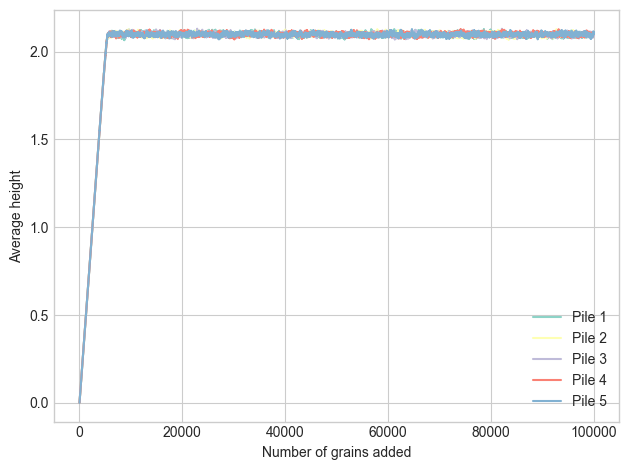
\includegraphics[width=0.9\textwidth]{figures/average_height.png}
	\caption{Average pile height against the number of grains added for five independent simulations.}
	\label{fig:average_height}
\end{figure}

As shown in Figure~\ref{fig:average_height}, the five piles show similar patterns. By about 10,000 grain additions, the average height has stabilised and fluctuates around 2.1. Therefore, I exclude the records from the first 10,000 additions as burn-in before further analysis.

\section{Avalanche Property Distributions}

After excluding the records from the first 10,000 additions, I use the remaining records to plot the observed frequencies of Topples, Area, Loss, and Length. I generate linear-scale, semi-log, and log-log plots for each of the four properties to explore their distribution shapes and identify candidate distributions for fitting. The linear-scale plots are shown in Figure~\ref{fig:linear} in Appendix~\ref{app:appendixA}.

\begin{figure}[htbp]
	\centering
	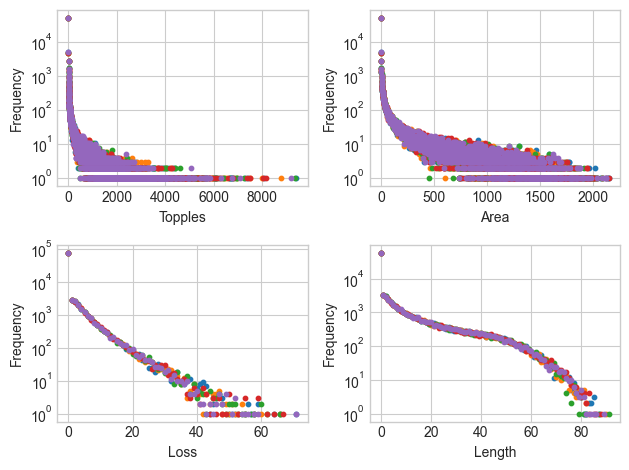
\includegraphics[width=0.49\textwidth]{figures/semi_log.png}
	\hfill
	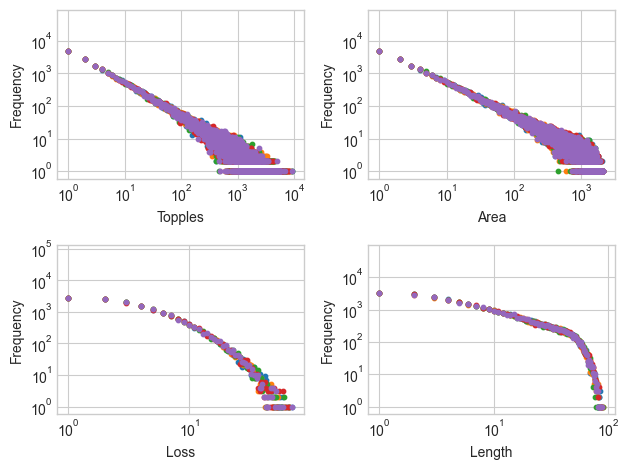
\includegraphics[width=0.49\textwidth]{figures/log_log.png}
	\caption{Observed frequencies of Topples, Area, Loss, and Length for five independent simulations on semi-log axes (left) and log-log axes (right).}
	\label{fig:distributions}
\end{figure}

As shown in Figure~\ref{fig:distributions}, the positive Loss values follow an approximately linear pattern on the semi-log plot, apart from deviations in the tail. Topples and Area show approximately linear patterns over part of their ranges on the log-log plot. However, Length does not follow a straight-line pattern on either plot.

Then I try to find a fit for the distribution for each of the avalanche properties.

\subsection{Topples}
Since Topples shows an approximately linear pattern on the log-log frequency plot, I consider a power law as a candidate distribution. I fit a power law to the observed frequencies and plot the fitted curve on the same scatter plot.

\begin{figure}[!htbp]
	\centering
	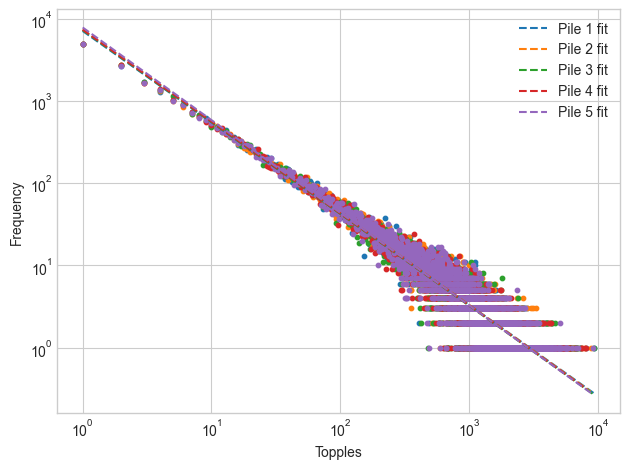
\includegraphics[width=0.6\textwidth]{figures/topples.png}
	\caption{Observed positive Topples frequencies and fitted power-law curves for five independent simulations on log-log axes.}
	\label{fig:dtopples}
\end{figure}

The five independent piles show similar patterns. The observed frequencies are distributed close to the fitted curves except in the tails. The estimated power-law exponent $\alpha$, MAE, and RMSE for each pile are shown in Table~\ref{tab:topples_fit}.

\begin{table}[htbp]
	\centering
	\begin{tabular}{cccc}
		\hline
		Pile & $\alpha$ & MAE & RMSE \\
		\hline
		1 & -1.1110 & 3.4764 & 47.1356 \\
		2 & -1.1174 & 3.8661 & 55.3308 \\
		3 & -1.1181 & 3.5590 & 52.4131 \\
		4 & -1.1185 & 3.7551 & 55.4676 \\
		5 & -1.1274 & 4.2641 & 64.2137 \\
		\hline
	\end{tabular}
	\caption{Estimated power-law exponents and fitting errors for Topples.}
	\label{tab:topples_fit}
\end{table}

The estimated exponents range from $-1.1274$ to $-1.1110$, showing little variation across the five piles. Additionally, MAE ranges from 3.4764 to 4.2641, while RMSE ranges from 47.1356 to 64.2137. The substantially larger RMSE indicates that some observed frequencies deviate considerably from the fitted values.

Overall, the observed Topples frequencies suggest approximate power-law behaviour, with fitted exponents close to $-1.12$, although deviations are present in the tails.

\subsection{Area}

Since the observed Area frequencies show an approximately linear pattern on the log-log plot, I first fit a power law, as for Topples. Similarly, I plot the fitted curve on the scatter plot and calculate MAE and RMSE. The fitted curves and fitting results are shown in Figure~\ref{fig:area_power} and Table~\ref{tab:area_power}. The fitted curve does not describe the trend of the observed frequencies well. I then fit a log-normal model to the observed frequencies and plot the fitted curve on the scatter plot.

\begin{figure}[htbp]
	\centering
	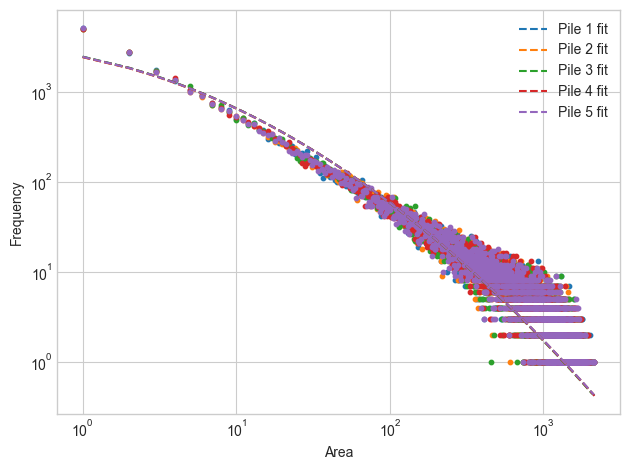
\includegraphics[width=0.6\textwidth]{figures/area_lognorm.png}
	\caption{Observed positive Area frequencies and fitted log-normal curves for five independent simulations on log-log axes.}
	\label{fig:area_lognorm}
\end{figure}

The fitted log-normal curves appear to describe the observed Area frequencies better. The estimated mean $\mu$ and variance $\sigma^2$ of $\log(\mathrm{Area})$, with MAE and RMSE for each pile, are shown in Table~\ref{tab:area_lognorm}.

\begin{table}[htbp]
	\centering
	\begin{tabular}{ccccc}
		\hline
		Pile & $\mu$ & $\sigma^2$ & MAE & RMSE \\
		\hline
		1 & 3.2215 & 4.8049 & 7.1053 & 68.8535 \\
		2 & 3.2310 & 4.8103 & 7.2480 & 69.0048 \\
		3 & 3.2138 & 4.7811 & 7.0596 & 66.6385 \\
		4 & 3.2267 & 4.7858 & 7.0092 & 66.9160 \\
		5 & 3.2295 & 4.8169 & 7.2742 & 69.8435 \\
		\hline
	\end{tabular}
	\caption{Estimated log-normal parameters and fitting errors for positive Area values.}
	\label{tab:area_lognorm}
\end{table}

It is worth noting that the MAE and RMSE for the power-law fit are about 16 and 257, respectively, which are much larger than those for the log-normal fit. Therefore, the log-normal model provides a better fit to the observed Area frequencies, with estimated parameters $\mu \approx 3.22$ and $\sigma^2 \approx 4.8$.


\subsection{Loss}

According to the semi-log plot of Loss frequencies above, the positive Loss values follow an approximately linear pattern. Therefore, I first fit a geometric distribution including zero. However, the fitted curves differ considerably from the observed frequencies, as shown in Figure~\ref{fig:loss_ge0}. I then fit a geometric distribution to only the positive Loss values, which gives a better fit.
\begin{figure}[htbp]
	\centering
	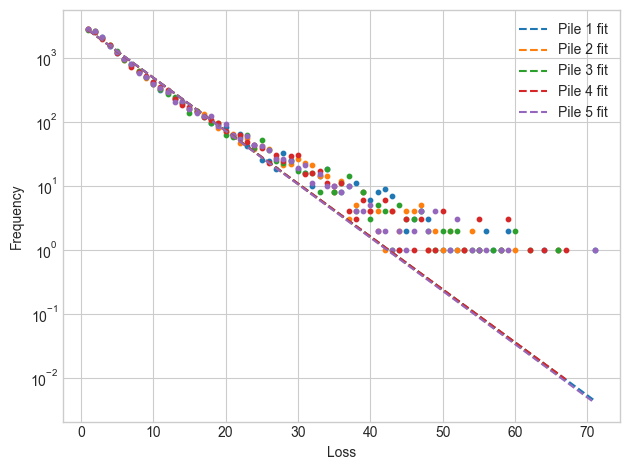
\includegraphics[width=0.6\textwidth]{figures/loss_geo.png}
	\caption{Observed positive Loss frequencies and fitted geometric curves for five independent simulations on semi-log axes.}
	\label{fig:loss_geo}
\end{figure}

Similarly, I calculate and record the estimated parameter $p$, MAE, and RMSE for each pile, as shown in Table~\ref{tab:loss_geo}.

\begin{table}[htbp]
	\centering
	\begin{tabular}{cccc}
		\hline
		Pile & $p$ & MAE & RMSE \\
		\hline
		1 & 0.1733 & 27.0177 & 59.4437 \\
		2 & 0.1741 & 28.8757 & 67.8951 \\
		3 & 0.1735 & 27.2988 & 62.3667 \\
		4 & 0.1732 & 28.6606 & 60.1797 \\
		5 & 0.1744 & 30.1436 & 68.4744 \\
		\hline
	\end{tabular}
	\caption{Estimated geometric distribution parameters and fitting errors for positive Loss values.}
	\label{tab:loss_geo}
\end{table}

Additionally, I fit a log-normal distribution to the positive Loss values. The fitted curves and fitting results are shown in Figure~\ref{fig:loss_lognorm} and Table~\ref{tab:loss_lognorm}. The fitted curves also appear to describe the observed frequencies well, but the RMSE is larger, while the MAE is similar.

Overall, the geometric distribution provides a better fit to the observed positive Loss frequencies in terms of RMSE, with an estimated parameter $p \approx 0.17$.

\newpage


\subsection{Length}
The observed Length frequencies do not show an approximately linear pattern on either the semi-log or log-log plot. I therefore explore a log-normal distribution as a candidate model. Using the same fitting process as for Area, I obtain the fitted curves shown alongside the observed positive Length frequencies in Figure~\ref{fig:length}.

\begin{figure}[htbp]
	\centering
	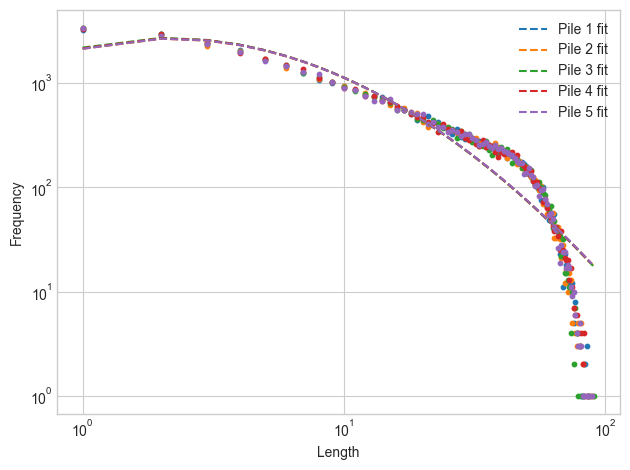
\includegraphics[width=0.6\textwidth]{figures/length.png}
	\caption{Observed positive Length frequencies and fitted log-normal curves for five independent simulations on log-log axes.}
	\label{fig:length}
\end{figure}

According to the figure above, there is a noticeable discrepancy between the fitted frequencies and the observed frequencies, though the fitted frequencies do provide a rough indication of the trend in the observed data.

Similarly, I calculate and record the estimated parameters $\mu$ and $\sigma^2$, together with MAE and RMSE for each pile, as shown in Table~\ref{tab:length}.

\begin{table}[htbp]
	\centering
	\begin{tabular}{ccccc}
		\hline
		Pile & $\mu$ & $\sigma^2$ & MAE & RMSE \\
		\hline
		1 & 2.1438 & 1.4079 & 89.6531 & 167.0913 \\
		2 & 2.1475 & 1.4166 & 93.1109 & 176.6598 \\
		3 & 2.1334 & 1.4183 & 90.0540 & 169.1877 \\
		4 & 2.1410 & 1.4138 & 86.4604 & 167.3350 \\
		5 & 2.1483 & 1.4174 & 88.8975 & 170.9569 \\
		\hline
	\end{tabular}
	\caption{Estimated log-normal parameters and fitting errors for positive Length values.}
	\label{tab:length}
\end{table}

Overall, the log-normal model with $\mu \approx 2.14$ and $\sigma^2 \approx 1.41$ provides a rough approximation to the distribution of positive Length values, although noticeable discrepancies remain.

\newpage

\section{Correlations Between Avalanche Properties}

In order to explore the relationships between the four avalanche properties, I first generate a pairwise scatter plot for Pile 1.

\begin{figure}[htbp]
	\centering
	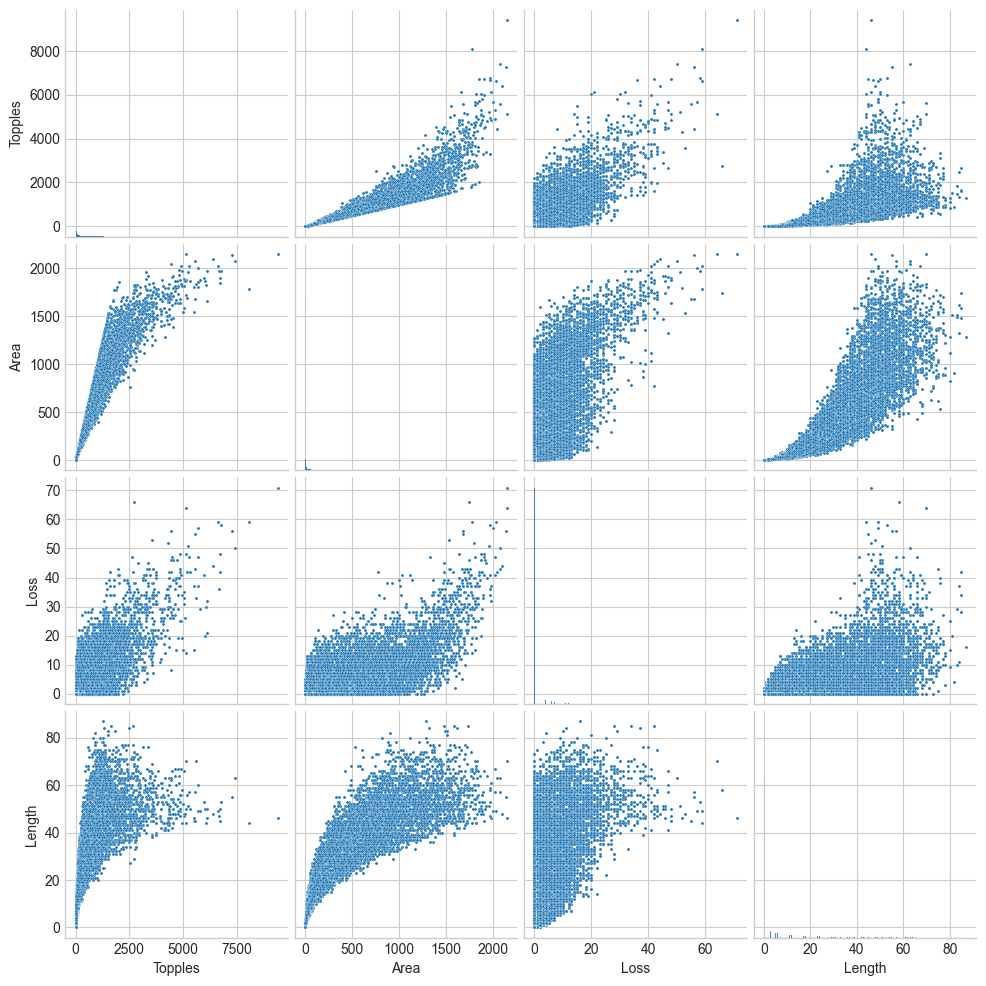
\includegraphics[width=0.6\textwidth]{figures/corr.png}
	\caption{Pairwise scatter plot of the four avalanche properties for Pile 1.}
	\label{fig:corr_1}
\end{figure}

As shown in Figure~\ref{fig:corr_1}, the relationships between the properties appear to be positive, with some showing non-linear patterns.

Therefore, I calculate the Spearman correlation coefficients for Pile 1 to quantify the strength of the monotonic relationships between the properties.

\begin{table}[htbp]
	\centering
	\begin{tabular}{lcccc}
		\hline
		& Topples & Area & Loss & Length \\
		\hline
		Topples & 1.000000 & 0.999919 & 0.626868 & 0.961980 \\
		Area    & 0.999919 & 1.000000 & 0.626550 & 0.962282 \\
		Loss    & 0.626868 & 0.626550 & 1.000000 & 0.626531 \\
		Length  & 0.961980 & 0.962282 & 0.626531 & 1.000000 \\
		\hline
	\end{tabular}
	\caption{Spearman correlation matrix for Pile 1.}
	\label{tab:corr_1}
\end{table}

The correlation matrices for Piles 2 to 5 are shown in Tables~\ref{tab:corr_2}, \ref{tab:corr_3}, \ref{tab:corr_4}, and \ref{tab:corr_5} in Appendix~\ref{app:appendixA}. The correlation coefficients for the same pair of properties are similar across all five piles.

Overall, Topples has very strong positive correlations with Area and Length, with coefficients above 0.9. Area and Length are also strongly positively correlated. Loss has lower positive correlations with the other properties, with coefficients around 0.63.


 